\documentclass[tikz,margin=3mm]{standalone}
\usepackage{amsmath}
\begin{document}
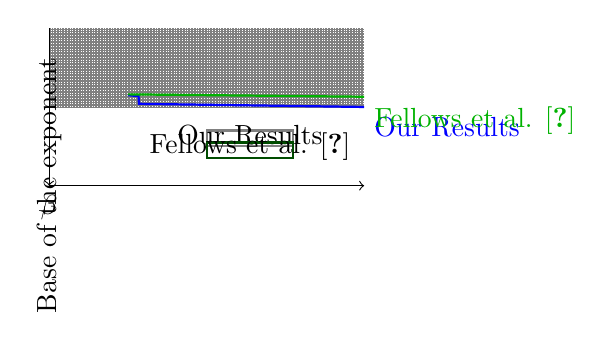
\begin{tikzpicture}

% Grid
\draw[style=help lines] (0,1) grid[step=0.02] (4,2);

% Axes
\draw[->] (0,2) -- (0,0) node[below] {$\beta$} coordinate (y轴);
\draw[->] (0,0) -- (4,0) node[below] {} coordinate (x轴);

% Labels
\node[rotate=90] at (y轴|-0.3,0) {Base of the exponent};

% Curves
\draw[blue,thick] (1,1.15) -- (1.135,1.137) -- (1.14,1.04) -- (4,1) node[below right] {Our Results};
\draw[green!70!black,thick] (1,1.16) -- (4,1.13) node[below right] {Fellows et al. \cite{fellows}};

% Legend
\draw[black!50!white,thick] (2,0.7) rectangle (3.1,0.5);
\draw (2.55,0.65) node {Our Results};
\draw[black!70!green,thick] (2,0.55) rectangle (3.1,0.35);
\draw (2.55,0.5) node {Fellows et al. \cite{fellows}};

\end{tikzpicture}
\end{document}